\chapter{VGA Display Driver}\label{chapter:VGA Display Driver}

\section{Overview}\label{section:Overview}
DaxOS initially used VGA text mode for its display. VGA text-mode is a part of the VGA standard and is available on most hardware.
However it is depreciated on newer systems in favor of the higher resolution VESA or GOP buffers on newer UEFI based systems.
The primary advantages of using VGA text-mode are:
\begin{enumerate}
    \item \textbf{ No need to worry about font-rendering}\\
    VGA text-mode abstracts away most of the complexity involved in writing a display driver including font management and rendering.
    \item \textbf{ Easy to program}\\
    Writing code to use VGA text-mode is as easy as writing characters to a particular memory address.
    \item \textbf{ No additional dependencies}\\
    You do not need an existing malloc() for instance.
\end{enumerate}

However there are also a couple of disadvantages:
\begin{enumerate}
    \item \textbf{ Low resolution}\\
    Text resolution is limited to about 25 lines of 80 character each.
    \pagebreak
    \item \textbf{ No drawing capability}\\
    It is not possible to draw pixels onto the screen in this mode.
    \item \textbf{ 16 color palette}\\
    Only 16 colors are available in this mode.
\end{enumerate}

\section{Printing text to the screen}\label{section:Printing text to the screen}
It is very simple to print text to the screen using VGA-text mode. The process basically involves writing the necessary 
character onto the VGA text-buffer. This buffer is located at \textbf{0xB8000}.\\

Every character to be displayed is represented by two bytes:
\begin{itemize}
    \item First byte determines the background and foreground color of the character.
    \item Second byte is the codepoint; i.e the character itself. 
\end{itemize}

Therefore to print the character `A' to the screen:

\lstset{language=C}
\begin{lstlisting}
    char *buffer = (char *)(intptr_t)0xB8000;
    *buffer++ = 12; \\bg is black, fg is white
    *buffer = 'A';
\end{lstlisting}

The actual display driver is much more sophisticated and involves a standardized API that the other parts of the OS can use.
\vspace{1cm}
\begin{figure}[h!]
	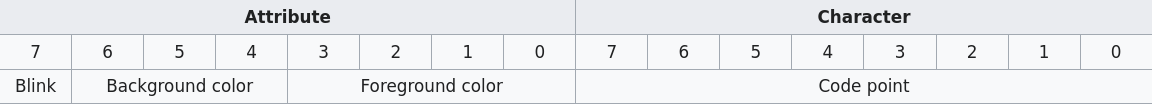
\includegraphics[width=\textwidth,height=\textheight,keepaspectratio]{vga_code}
	\caption{VGA representation for a single character}
\end{figure}
\pagebreak

\section{Display Driver API}\label{section:Display Driver API}
The display driver supports the following API calls:
\begin{lstlisting}
    void tty_initialize(void);
    void tty_put_char(char c);
    void tty_write(const char *data, size_t size);
    void tty_write_string(const char *data);
    void tty_write_string_centered(const char *string);
    void tty_print_horizontal_rule(const char symbol);
    void tty_setcolor(uint8_t color);
    void tty_print_success(const char *string, const char *success_string);
\end{lstlisting}

\vspace{1.5cm}
\begin{figure}[h!]
	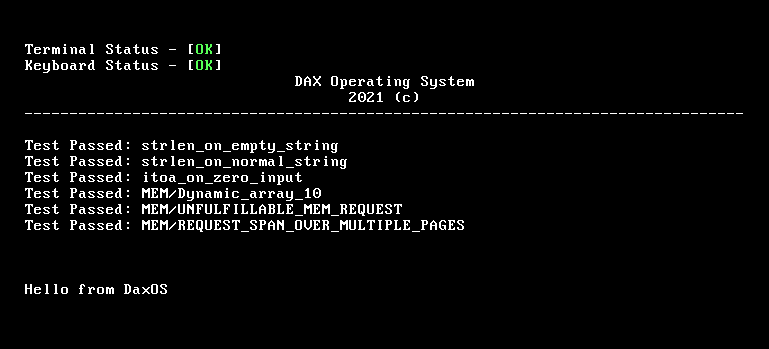
\includegraphics[width=\textwidth,height=\textheight,keepaspectratio]{vga}
	\caption{VGA display driver running in DaxOS}
\end{figure}